\section{Background on LDA}
\label{sec:background}

%------------------------------------------------

Topic modeling, a form of latent variable modeling, is an unsupervised machine learning method which attempts to recreate the distribution of so-called ``topics'' an author used to generate a corpus of documents.
The term topic is used to describe a frequency distribution of terms within a vocabulary.
In this use, a topic can be understood to represent an academic concept covered within the context of a course.
This is based on the assumption that the words used in a course description when introducing the course's topics are the same words used within descriptions of the topic itself.
The topics discovered in a corpus can be used to categorize documents and provide structure to an otherwise unknown dataset.

%------------------------------------------------

\acf{lda} is a specific type of topic modeling which assumes that a mixture of multiple topics exist within a single document in some proportion (\ie\ were used to generate that document)~\cite{Blei2003}.
\ac{lda} assumes a generative process where, for each word in the document, the algorithm selects a distribution over topics, selects a topic, and then selects a vocabulary term~\cite{Blei2003}.
Reversing this generative process is significantly more difficult because the topic distributions are unknown; these unknown information is what the ``hidden model'' or ``latent model'' refers to.

%------------------------------------------------

The computation \ac{lda} performs is the determination of the topic distributions over a set of documents.
Given the set of documents as input, generating the corpus topics is a probabilistic process.
Taking the variables $\theta_{d,k}$ (topic proportion for topic $k$ in document $d$), $\beta_{1:k}$ (topic $k$), $z_{d,n}$ (topic assignment for word $n$ in document $d$), and $w_{d,n}$ (the $n^{th}$ word in document $d$), \ac{lda} estimates the posterior probability in \eref{eq:posterior}~\cite{Blei2012}.

%------------------------------------------------

\begin{equation}
p(\beta_{1:K}, \theta_{1:D},z_{1:D} | w_{1:D}) = \frac{\beta_{1:K},
\theta_{1:D},z_{1:D}, w_{1:D}}{w_{1:D}}
\label{eq:posterior}
\end{equation}

%------------------------------------------------

\noindent
Gibbs Sampling is used to estimate the denominator (\ie\ the evidence)~\cite{Blei2003}.
Running \ac{lda} over a document set results in a usable set of vocabulary frequency distributions or topics for each document.

%------------------------------------------------

A graphical ``plate'' diagram of \ac{lda}'s generative process is given in \fref{fig:lda-plates}, adapted from~\cite{Blei2003}.
Circular nodes represent random variables while rectangular plates represent duplication.
The shaded node is the only observed (\ie\ evidence) variable, words from the document set.

%------------------------------------------------

\begin{figure}
  \centering
  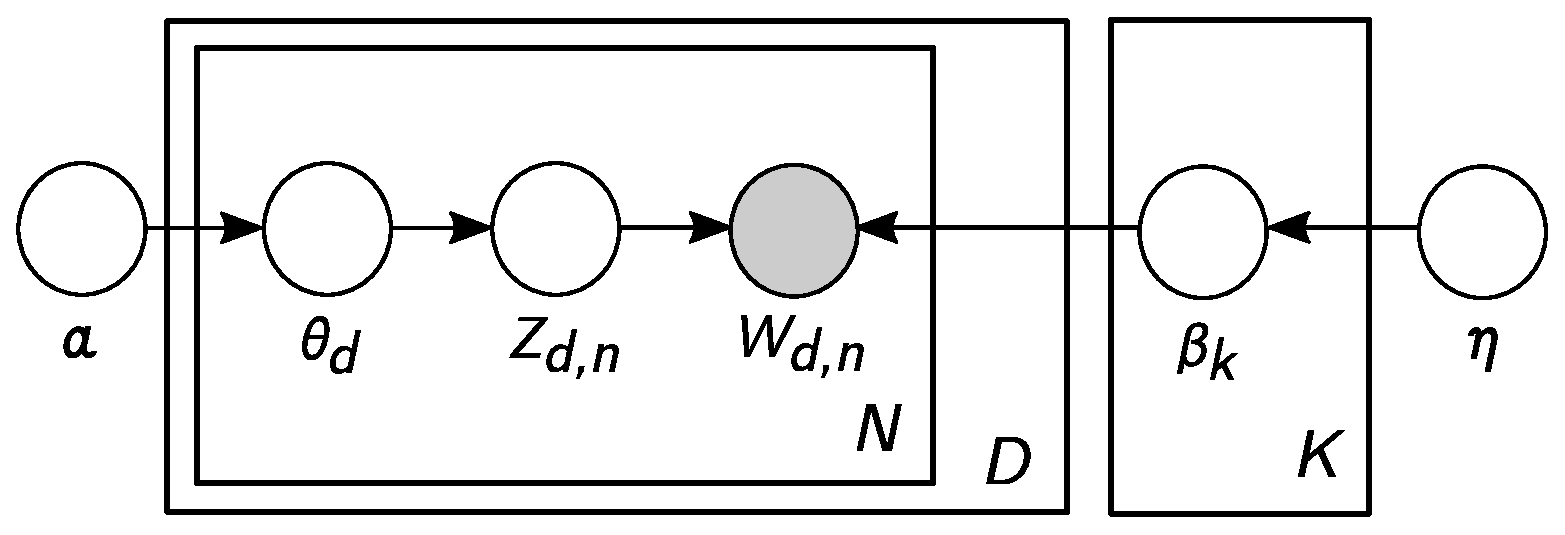
\includegraphics[width=0.45\textwidth]{figures/lda-plates}
  \caption{LDA graphical diagram adapted from~\cite{Blei2012}\label{fig:lda-plates}.}
\end{figure}

%------------------------------------------------

\subsection{Related Work}
\label{sec:related-work}

%------------------------------------------------

Our research complements other efforts within Computer Science education that are directed towards categorization of content to improve pedagogy, \eg\ Hubwieser et al.~\cite{hubwieser2013}.
We believe that our project contributes both, by identifying content (\ie\ topics) being taught across institutions and by identifying gaps and unique contributions.
This information can be compared to teacher competencies and used to design assessment and instruments to measure them.
Another area in which this work can assist is in identification of concepts and their classification, especially ``threshold concepts''~\cite{ShinnersKennedyFincher2013}.
Overall, we believe our data-driven approach complements other qualitative efforts by building on them and by automating some aspects of the research.

%------------------------------------------------

Other work has also attempted to extract concept information from course data.
Yang et al.\ employ four distinct techniques to map courses into a conceptual space and then learn prerequisite relationships between similar courses~\cite{Yang2015}.
Two of their conceptual mapping techniques generate latent features, which have the downside of not being human-readable as in \ac{lda}.
The remaining two techniques generate human-readable topics, but rely either on an outside source (Wikipedia) or simply represent concepts as the vocabulary of the document.
The benefit of \ac{lda} as an information retrieval tool is its ability to generate pseudo human-readable topics while acting in a fully unsupervised manner on a single, large data set.
Our approach naively targets a dataset of fixed universities and customizes web scrapers specifically for their computer science departments.
Effland et al.\ introduces a robust web crawler system to automatically search for, identify, and extract course descriptions from disparate locations on the Internet~\cite{Effland2015}.
Application of similar technology in this work was considered, and would greatly improve the scale of the analyzed data.

%------------------------------------------------

